\documentclass[12pt,a4paper]{article}
\usepackage{luatexja}
\usepackage{luatexja-fontspec}
\usepackage{fontspec}
\usepackage{graphicx}
\usepackage{subcaption}
\usepackage{listings}
\usepackage[margin=2.5cm]{geometry}
\usepackage[hidelinks]{hyperref}

% ===== 在原始模板基础上补充 =====
\usepackage{booktabs}
\usepackage{multirow}
\usepackage{makecell}
\usepackage{array}
\usepackage{float}
\usepackage{caption}
\usepackage{amsmath,amssymb,bm}
\usepackage{xcolor}
\usepackage{tikz}
\usetikzlibrary{arrows.meta,positioning,shapes.geometric,fit,calc}
\usepackage{enumitem}
\usepackage{url}
\usepackage{indentfirst}

\lstset{
    basicstyle=\ttfamily\footnotesize,
    breaklines=true,
    frame=single
}

\graphicspath{{images/}}
\setmainjfont{Noto Serif CJK SC}[
    BoldFont=Noto Serif CJK SC Bold,
    ItalicFont=Noto Serif CJK SC Light,
]
\setmainfont{Times New Roman}
\setsansjfont{Noto Sans CJK SC}[
    BoldFont=Noto Sans CJK SC Bold,
]

\linespread{1.35}
\setlength{\parindent}{2em}
\captionsetup{font=small,labelfont=bf}
\renewcommand{\contentsname}{目录}
\emergencystretch=1em
\setlist{nosep,leftmargin=2em}

% 截图占位：把图片放到 images/ 下同名文件即可自动替换
\newcommand{\screenshot}[2]{%
  \IfFileExists{images/#1}%
    {\includegraphics[width=0.92\linewidth]{#1}}%
    {\fbox{\parbox[c][0.28\textheight][c]{0.86\linewidth}{\centering
      \textbf{待补截图}\\[4pt] #2}}}%
}

\title{\textbf{基于空域-频域联合分析的\\深度伪造检测与可解释系统}}
\author{课程设计小组}
\date{\today}

\begin{document}

% 封面：南京信息工程大学课程设计报告
% 作为 main.tex 的片段使用：% 封面：南京信息工程大学课程设计报告
% 作为 main.tex 的片段使用：% 封面：南京信息工程大学课程设计报告
% 作为 main.tex 的片段使用：\input{cover}
% 也可用 cover_standalone.tex 单独编译预览
% 所有字段都可在下面几行改：
\def\reporttype{课程设计报告}
\def\reporttitle{基于空域-频域联合分析的深度伪造检测与可解释系统}
\def\studentname{付学瑞}
\def\studentid{202383290286}
\def\major{信息安全}
\def\college{网络空间安全学院}
\def\advisor{}
\def\coversdate{二○二六年十二月}

\begin{titlepage}
\centering
\vspace*{0.9cm}


\includegraphics[width=10.4cm]{uni_name.png}\\[1.0cm]

{\sffamily\bfseries\fontsize{24}{30}\selectfont \reporttype}\\[1.0cm]


\includegraphics[width=3.3cm]{logo.png}\\[1.4cm]

{\fontsize{14}{22}\selectfont
\renewcommand{\arraystretch}{1.75}
\begin{tabular}{r@{\hspace{8pt}}c}
\makebox[3.0cm][r]{\sffamily 题\quad 目} &
  \underline{\makebox[9.1cm][c]{\fontsize{11}{14}\selectfont \reporttitle}} \\[2pt]
\makebox[3.0cm][r]{\sffamily 学生姓名：} &
  \underline{\makebox[9.1cm][c]{\studentname}} \\[2pt]
\makebox[3.0cm][r]{\sffamily 学\qquad 号：} &
  \underline{\makebox[9.1cm][c]{\studentid}} \\[2pt]
\makebox[3.0cm][r]{\sffamily 专\qquad 业：} &
  \underline{\makebox[9.1cm][c]{\major}} \\[2pt]
\makebox[3.0cm][r]{\sffamily 学\qquad 院：} &
  \underline{\makebox[9.1cm][c]{\college}} \\[2pt]
\makebox[3.0cm][r]{\sffamily 指导教师：} &
  \underline{\makebox[9.1cm][c]{\advisor}} \\
\end{tabular}}

\vfill
{\fontsize{15}{20}\selectfont \coversdate}
\vspace{1.0cm}
\end{titlepage}

% 也可用 cover_standalone.tex 单独编译预览
% 所有字段都可在下面几行改：
\def\reporttype{课程设计报告}
\def\reporttitle{基于空域-频域联合分析的深度伪造检测与可解释系统}
\def\studentname{付学瑞}
\def\studentid{202383290286}
\def\major{信息安全}
\def\college{网络空间安全学院}
\def\advisor{}
\def\coversdate{二○二六年十二月}

\begin{titlepage}
\centering
\vspace*{0.9cm}


\includegraphics[width=10.4cm]{uni_name.png}\\[1.0cm]

{\sffamily\bfseries\fontsize{24}{30}\selectfont \reporttype}\\[1.0cm]


\includegraphics[width=3.3cm]{logo.png}\\[1.4cm]

{\fontsize{14}{22}\selectfont
\renewcommand{\arraystretch}{1.75}
\begin{tabular}{r@{\hspace{8pt}}c}
\makebox[3.0cm][r]{\sffamily 题\quad 目} &
  \underline{\makebox[9.1cm][c]{\fontsize{11}{14}\selectfont \reporttitle}} \\[2pt]
\makebox[3.0cm][r]{\sffamily 学生姓名：} &
  \underline{\makebox[9.1cm][c]{\studentname}} \\[2pt]
\makebox[3.0cm][r]{\sffamily 学\qquad 号：} &
  \underline{\makebox[9.1cm][c]{\studentid}} \\[2pt]
\makebox[3.0cm][r]{\sffamily 专\qquad 业：} &
  \underline{\makebox[9.1cm][c]{\major}} \\[2pt]
\makebox[3.0cm][r]{\sffamily 学\qquad 院：} &
  \underline{\makebox[9.1cm][c]{\college}} \\[2pt]
\makebox[3.0cm][r]{\sffamily 指导教师：} &
  \underline{\makebox[9.1cm][c]{\advisor}} \\
\end{tabular}}

\vfill
{\fontsize{15}{20}\selectfont \coversdate}
\vspace{1.0cm}
\end{titlepage}

% 也可用 cover_standalone.tex 单独编译预览
% 所有字段都可在下面几行改：
\def\reporttype{课程设计报告}
\def\reporttitle{基于空域-频域联合分析的深度伪造检测与可解释系统}
\def\studentname{付学瑞}
\def\studentid{202383290286}
\def\major{信息安全}
\def\college{网络空间安全学院}
\def\advisor{}
\def\coversdate{二○二六年十二月}

\begin{titlepage}
\centering
\vspace*{0.9cm}


\includegraphics[width=10.4cm]{uni_name.png}\\[1.0cm]

{\sffamily\bfseries\fontsize{24}{30}\selectfont \reporttype}\\[1.0cm]


\includegraphics[width=3.3cm]{logo.png}\\[1.4cm]

{\fontsize{14}{22}\selectfont
\renewcommand{\arraystretch}{1.75}
\begin{tabular}{r@{\hspace{8pt}}c}
\makebox[3.0cm][r]{\sffamily 题\quad 目} &
  \underline{\makebox[9.1cm][c]{\fontsize{11}{14}\selectfont \reporttitle}} \\[2pt]
\makebox[3.0cm][r]{\sffamily 学生姓名：} &
  \underline{\makebox[9.1cm][c]{\studentname}} \\[2pt]
\makebox[3.0cm][r]{\sffamily 学\qquad 号：} &
  \underline{\makebox[9.1cm][c]{\studentid}} \\[2pt]
\makebox[3.0cm][r]{\sffamily 专\qquad 业：} &
  \underline{\makebox[9.1cm][c]{\major}} \\[2pt]
\makebox[3.0cm][r]{\sffamily 学\qquad 院：} &
  \underline{\makebox[9.1cm][c]{\college}} \\[2pt]
\makebox[3.0cm][r]{\sffamily 指导教师：} &
  \underline{\makebox[9.1cm][c]{\advisor}} \\
\end{tabular}}

\vfill
{\fontsize{15}{20}\selectfont \coversdate}
\vspace{1.0cm}
\end{titlepage}


\section*{摘要}
\addcontentsline{toc}{section}{摘要}

\noindent
深度伪造技术已从早期的自编码器换脸发展到扩散模型生成与商用工具一键换脸，伪造内容的逼真度与获取门槛同时恶化。现有检测方法在单一数据集上准确率很高，但在跨数据集、强压缩以及训练时未见过的生成方法上性能急剧下降。本文以“检测器到底学到了什么”为核心问题，构建了一套可复现的图像级检测与评测流程：以 FaceForensics++ C23 的 580 个身份、约 3.5 万张人脸帧训练 ResNet18 基线，在 Celeb-DF 上做跨库测试，并系统评测 JPEG 压缩、噪声、模糊、下采样、裁剪等退化。在此基础上实现了 RGB + FFT + SRM 的双流结构与质量感知门控，通过消融实验发现频域分支未带来稳定收益、门控退化为常数；平均频谱分析表明真假图的频域差异主要来自压缩块效应而非生成器指纹，留出一种伪造方法的开集实验（未见 FaceShifter，AUC 0.598）也印证了捷径学习。最终系统以 FastAPI 实现，提供伪造概率、Grad-CAM 热图、频谱图和带哈希链审计的 PDF 报告，单图推理约 11 ms。本文的主要价值不在于刷新指标，而在于用受控实验定位了“同库高指标、跨域失效”的成因，并给出了可复现的评测协议。

\vspace{1em}
\noindent\textbf{关键词：}深度伪造检测；频域分析；跨库泛化；捷径学习；可解释性

\newpage
\section*{Abstract}
\addcontentsline{toc}{section}{Abstract}

\noindent
Deepfake technology has evolved from early autoencoder-based face swapping to diffusion-based
synthesis and one-click commercial tools, making forged content both more realistic and easier to
produce. Existing detectors achieve high accuracy on a single dataset but degrade sharply under
cross-dataset shifts, heavy compression, and unseen generators. This report investigates what a
detector actually learns. We build a reproducible image-level pipeline: a ResNet18 RGB baseline
trained on 580 identities (about 35k face frames) from FaceForensics++ C23, evaluated on Celeb-DF
for cross-dataset generalization and on six degradations. We further implement a dual-stream model
with FFT magnitude and SRM residual branches plus a quality-aware gate. Ablations show no stable
gain from the frequency branch, and the gate collapses to a constant (0.4272 $\pm$ 0.0008).
Mean-spectrum analysis indicates that the real/fake difference is dominated by axis-aligned
compression artifacts rather than generator fingerprints; an open-set experiment that holds out
FaceShifter yields AUC 0.598 despite 0.933 in-domain AUC. The final system, built with FastAPI,
returns a forgery score, a Grad-CAM heatmap, a spectrum image, and a PDF report with a
hash-chained audit log; single-image inference takes about 11 ms on GPU and 37 ms on CPU.

\vspace{1em}
\noindent\textbf{Keywords:} deepfake detection; frequency analysis; cross-dataset generalization;
shortcut learning; interpretability

\newpage
\tableofcontents
\newpage

\section{绪论}

\subsection{研究背景}

\subsubsection{生成技术的快速演进}

深度伪造（Deepfake）指利用深度学习生成或篡改人脸、语音等内容的技术。2014 年生成对抗网络（GAN）\cite{goodfellow2014gan} 提出后，换脸、表情重演、全脸合成、属性编辑四类技术相继成熟。2019 年的 FaceForensics++ 数据集用 4 种方法生成了数千条伪造视频\cite{rossler2019ffpp}；此后 FaceShifter\cite{li2020faceshifter}、SimSwap、FaceDancer 等方法不断降低伪造门槛；2022 年以来，以 Stable Diffusion 为代表的扩散模型\cite{rombach2022ldm} 把全脸合成的逼真度推到新高度；DeepFaceLab、HeyGen 等商用工具更是让非专业用户只需一张照片和一段音频就能生成以假乱真的视频。

生成技术的演进呈现三个趋势：\textbf{方法多样化}（从单一换脸到换脸、重演、合成、编辑并存）、\textbf{质量真实化}（混合边界、光照一致性越来越难被肉眼识别）、\textbf{门槛平民化}（开源工具与在线服务）。这三者共同导致检测方的“先验假设”不断失效。DF40 基准\cite{yan2024df40} 已收录 40 种伪造方法，是 FF++ 的 10 倍，并明确指出 FF++ 的伪造方法已过时四年。

\subsubsection{安全威胁}

深度伪造的滥用已造成实际损失：冒充企业高管进行视频会议诈骗、伪造名人言论制造舆论、生成色情内容进行敲诈、伪造证据干扰司法等。据公开报道，2024 年香港一家公司曾因 AI 换脸视频会议被骗走约 2 亿港元。伪造内容的传播还会侵蚀“眼见为实”的社会信任基础，其危害已超出个人层面。

\subsubsection{法规与治理背景}

我国对深度合成与生成式内容的治理走在世界前列：

\begin{itemize}
  \item 《互联网信息服务深度合成管理规定》，2022 年 11 月公布，\textbf{2023 年 1 月 10 日施行}，要求深度合成服务提供者对生成内容进行标识、建立辟谣机制\cite{cac2022deepsynth}；
  \item 《生成式人工智能服务管理暂行办法》，2023 年 8 月 15 日施行，明确服务提供者的内容安全责任\cite{cac2023genai}；
  \item 《人工智能生成合成内容标识办法》，2025 年 3 月公布，\textbf{2025 年 9 月 1 日施行}，配套强制性国家标准，要求对 AI 生成合成内容添加显式或隐式标识\cite{cac2025label}。
\end{itemize}

法规落地依赖技术手段：标识可以被移除或篡改，平台仍需具备“内容真实性鉴别”能力。因此检测技术不是可选项，而是治理链条中的基础设施。

\subsubsection{技术挑战}

从检测方视角看，困难集中在六个方面：

\begin{enumerate}
  \item \textbf{来源异构}：不同数据集、不同平台、不同拍摄设备的内容分布差异巨大；
  \item \textbf{生成模型迭代快}：训练时见过的伪造方法，几个月后可能已被淘汰；
  \item \textbf{伪造类型多样}：换脸、重演、全脸合成、属性编辑的伪影形态完全不同；
  \item \textbf{真实场景退化}：压缩、噪声、低分辨率、裁剪在传播链中几乎必然发生；
  \item \textbf{标注稀缺}：新伪造方法出现时没有标注数据，监督学习难以及时跟进；
  \item \textbf{可解释与合规}：判定结果需要能被人理解、能审计，才能用于申诉与追责。
\end{enumerate}

\subsection{国内外研究现状}

国际上，深度伪造检测经历了从“手工特征 + 浅层分类器”到“深度网络端到端”的转变。早期 MesoNet\cite{afchar2018mesonet}、Xception\cite{rossler2019ffpp} 等直接对 RGB 图像做二分类；随后研究者发现伪造过程会在频域留下痕迹，F3-Net\cite{qian2020f3net}、SPSL\cite{liu2021spsl}、SRM\cite{luo2021srm} 等方法引入 DCT/FFT 与高通滤波；RECCE\cite{cao2022recce}、DIRE\cite{wang2023dire}、AEROBLADE\cite{ricker2024aeroblade} 等转向“重构误差”；UnivFD\cite{ojha2023univfd} 等则利用 CLIP 的通用视觉表示提升跨生成器泛化。评测方面，FaceForensics++、Celeb-DF、DFDC、ForgeryNet、GenImage、DF40 等数据集推动了协议标准化，DeepfakeBench\cite{yan2023deepfakebench} 则统一了 15 种检测器的实现与评测。

国内高校与企业在该方向同样活跃：中国科学技术大学张勇东、谢洪涛团队提出身份一致性 Transformer（CVPR 2022）\cite{dong2022ict} 与多模态人脸篡改检测方法；西安交通大学蔺琛皓、沈超、管晓宏等在《计算机学报》发表虚假数字人脸内容生成与检测技术综述\cite{lin2023survey}；西安电子科技大学高新波团队近年转向大模型时代的多模态伪造检测；腾讯优图实验室参与构建了 DF40 基准。总体而言，国内工作在国际顶会/顶刊上已占相当比例，且在“多模态”“可解释”“治理”等方向有特色布局。

\subsection{检测性能的公开水平}

从公开结果看，FF++ c23 二分类的准确率通常在 95\%--99\% 之间：Xception 约 95.7\%\cite{rossler2019ffpp}，
F3-Net 约 97.5\%\cite{qian2020f3net}，SPSL 接近 99\%\cite{liu2021spsl}，AUC 多在 0.96 以上。
跨库到 Celeb-DF 时性能明显下降，AUC 通常落在 0.70--0.90，身份一致性方法报告约 0.86\cite{dong2022ict}。
需要注意的是，这些数字大多基于全量 FF++（数十万到百万级训练帧）、更强的 backbone 以及视频级评测，
与本文的小规模、身份隔离、帧级设置不可直接比较。本文在 3,600 帧测试集上取得 85.6\% 的准确率
（阈值 0.5）与 0.933 的帧级 AUC，跨库 AUC 0.716，处于公开结果的较低区间，原因在第 5.9 节分析。

\subsection{本文主要工作}

本文不追求在单一数据集上刷高指标，而是围绕“检测器学到了什么、为什么换场景就失效”做系统性的工程与实验：

\begin{enumerate}
  \item \textbf{构建可复现的数据与评测管线}：从 FF++ C23 按身份抽样 580 个训练身份、约 4 万张人脸帧，按源视频 id 划分训练/验证/测试，杜绝身份泄漏；引入 Celeb-DF 作为跨库测试，自行生成 6 类退化。
  \item \textbf{实现 RGB 基线、双流与质量门控}：RGB 分支用 ResNet18 迁移学习，频域分支用 log$|$FFT$|$ 幅度谱 + SRM 噪声残差，门控用高频能量作为质量代理。
  \item \textbf{系统消融与负结果分析}：通过“有门控/无门控/纯 RGB”的对照、门控值统计、平均频谱差异、高频能量分布，定位频域分支无效与门控退化的原因。
  \item \textbf{多维度评测}：同库、视频级聚合、跨库、8 种退化矩阵、留出一种伪造方法的开集实验，并统一“部署口径/排序口径”两套阈值报告方式。
  \item \textbf{可解释性与系统落地}：Grad-CAM + 频谱图 + deletion/insertion 定量验证；FastAPI 服务提供 PDF 报告与哈希链审计日志。
\end{enumerate}

\subsection{报告结构}

第 2 章综述生成技术、检测方法、数据集与现有问题；第 3 章介绍数据与评测协议；第 4 章给出模型与训练方法；第 5 章报告实验与分析；第 6 章介绍系统实现；第 7 章总结并展望。

\section{相关工作}

\subsection{深度伪造生成技术}

按照 DF40 基准的分类\cite{yan2024df40}，深度伪造可分为四类。

\textbf{换脸（Face-Swapping, FS）}：把源人脸的身份迁移到目标视频。早期 DeepFakes 类方法依赖“编码器-解码器 + 掩码融合”，会在人脸与背景交界处留下混合伪影；FaceShifter\cite{li2020faceshifter}、SimSwap、FaceDancer、BlendFace 等新方法通过身份-背景解耦直接生成整幅图像，\textbf{不再有显式的混合步骤}——这直接瓦解了“检测混合边界”这一类方法的假设。

\textbf{表情重演（Face-Reenactment, FR）}：驱动目标人物做出源人物的表情或口型，代表方法有 Face2Face\cite{thies2016face2face}、NeuralTextures\cite{thies2019neural}、FOMM、SadTalker、Wav2Lip 等。重演类伪造通常不替换身份，只在局部改变纹理与几何，伪影更弱，是检测的难点。

\textbf{全脸合成（Entire Face Synthesis, EFS）}：从噪声直接生成不存在的人脸，代表方法有 StyleGAN 系列、VQGAN、DDPM\cite{ho2020ddpm}、Stable Diffusion\cite{rombach2022ldm}、PixArt-$\alpha$、DiT 等。扩散模型生成的图像在频域上更接近真实分布，传统基于 GAN 指纹的检测器容易失效。

\textbf{属性编辑（Face Editing, FE）}：修改年龄、性别、表情等属性，如 StarGAN、StyleCLIP、e4e 等。

从检测角度看，生成技术的演进带来两个关键变化：\textbf{伪影从“结构性”转向“统计性”}（从明显的融合边界，变成难以人眼察觉的频域/噪声分布差异），\textbf{方法从“少数几种”变成“持续涌现”}（DF40 已收录 40 种方法，远超 FF++ 的 4 种）。

\subsection{深度伪造检测方法}

\subsubsection{空域方法}

最直接的思路是把检测当作图像二分类。MesoNet\cite{afchar2018mesonet} 用浅层卷积捕捉局部纹理；FaceForensics++ 提出的 Xception 基线\cite{rossler2019ffpp} 成为此后多年的标准 backbone；Multi-attentional 方法\cite{zhao2021multi} 用多注意力头捕捉不同区域的伪影；身份一致性 Transformer\cite{dong2022ict} 则显式建模“源身份与目标身份”的一致性，在跨库场景表现较好。

空域方法的优点是实现简单、推理快，缺点是容易学到与数据集相关的捷径（压缩方式、人脸对齐方式、身份分布），跨库时性能下降明显。

\subsubsection{频域方法}

伪造过程中的上采样、插值、生成器上采样层会在频域留下规律性痕迹，因此频域方法成为一条重要分支：

\begin{itemize}
  \item \textbf{F3-Net}\cite{qian2020f3net}：用 DCT 提取频域特征，并与 RGB 特征融合；
  \item \textbf{SPSL}\cite{liu2021spsl}：发现相位谱包含更丰富的伪造线索，提出空间-相位双流；
  \item \textbf{SRM}\cite{luo2021srm}：用 SRM 高通滤波器提取噪声残差，抑制图像内容、突出伪造噪声。
\end{itemize}

频域方法的共同假设是“伪造会留下稳定的频域指纹”。但这一假设在强压缩下是否成立，文献中讨论不足。本文的实验（第 5 章）发现，FF++ C23 上真假图的平均频谱差异主要集中在水平/垂直轴，呈压缩块效应形态，提示频域分支学到的可能更多是“压缩方式”而非“生成器指纹”。

\subsubsection{重构与解耦方法}

这类方法不直接分类，而是先“重建”再比较：RECCE\cite{cao2022recce} 用重构-分类联合学习，把远离真实特征聚类中心的样本判为伪造；DIRE\cite{wang2023dire} 用预训练扩散模型重建输入图像，以重建误差作为伪造线索；AEROBLADE\cite{ricker2024aeroblade} 利用潜扩散模型自编码器的重建误差，无需训练即可检测扩散生成图像。重构类方法的优势是\textbf{对未见生成器更鲁棒}，因为它们建模的是“真实图像流形”，而不是某类伪造的判别边界；缺点是对非扩散生成的伪造（如换脸）不一定适用，且推理成本高。

\subsubsection{通用视觉表示方法}

UnivFD\cite{ojha2023univfd} 发现，冻结的 CLIP 视觉编码器 + 线性分类器在跨生成器场景下优于专门训练的检测器。这类方法把“检测”转化为“真实图像与生成图像在通用语义空间中的分布差异”，泛化性较好，但对压缩、低分辨率等退化的鲁棒性仍需验证。

\subsubsection{数据增广与自监督方法}

为缓解“新伪造方法没有标注”的问题，SBI\cite{shiohara2022sbi} 用自混合（self-blending）合成大量伪训练样本，让模型学习“混合边界”这类通用线索；也有工作用自监督预训练、对比学习提升特征的可迁移性。本文的实验表明，仅靠随机退化增广不足以带来强压缩下的鲁棒性。

\subsubsection{时序与多模态方法}

视频检测可利用帧间一致性、眨眼频率、光流等时序线索；多模态方法进一步融合音频、文本、元数据。FakeAVCeleb、AV-Deepfake1M 等数据集推动了这一方向。本文聚焦图像级检测，时序与多模态仅作为展望。

表~\ref{tab:methods} 对上述路线做了汇总。

\begin{table}[H]
\centering
\caption{检测方法路线对比}
\label{tab:methods}
\small
\begin{tabular}{p{2.0cm}p{4.0cm}p{4.3cm}p{3.4cm}}
\toprule
路线 & 代表工作 & 核心思想 & 主要局限 \\
\midrule
空域 & MesoNet, Xception, 多注意力, ICT & 直接学习纹理/身份不一致 & 易学数据集捷径，跨库掉点 \\
频域 & F3-Net, SPSL, SRM & 伪造留下频域/噪声指纹 & 强压缩下高频信息被破坏 \\
重构 & RECCE, DIRE, AEROBLADE & 用重建误差衡量“像不像真实图像” & 依赖大模型，推理贵，对换脸不一定适用 \\
通用表示 & UnivFD & 冻结 CLIP + 线性分类器 & 对退化鲁棒性待验证 \\
数据增广 & SBI & 自混合合成伪样本 & 依赖混合假设，新式换脸无混合 \\
时序/多模态 & 各类视频/音视频方法 & 利用帧间与跨模态一致性 & 数据与算力门槛高 \\
\bottomrule
\end{tabular}
\end{table}

\subsection{数据集与评测基准}

\begin{table}[H]
\centering
\caption{常用深度伪造数据集}
\label{tab:datasets}
\small
\begin{tabular}{p{2.6cm}p{1.2cm}p{5.6cm}p{4.4cm}}
\toprule
数据集 & 年份 & 规模与特点 & 常见用途 \\
\midrule
FaceForensics++\cite{rossler2019ffpp} & 2019 & 1,000 真 + 6,000 假视频，4 种方法，c23/c40/raw 三档压缩 & 训练集、同库评测 \\
Celeb-DF\cite{li2020celebd} & 2020 & 590 真 + 5,639 假视频，换脸质量更高 & 跨库测试 \\
DFDC\cite{dolhansky2020dfdc} & 2020 & 10 万+ 视频，真实场景、多人脸 & 大规模竞赛 \\
ForgeryNet\cite{he2021forgerynet} & 2021 & 15 种方法、百万级图像/视频 & 大规模训练 \\
GenImage\cite{zhu2023genimage} & 2023 & 8 种生成器、百万级图像 & AIGC 图像检测 \\
DF40\cite{yan2024df40} & 2024 & 40 种方法（换脸/重演/合成/编辑） & 下一代评测基准 \\
\bottomrule
\end{tabular}
\end{table}

评测基准方面，DeepfakeBench\cite{yan2023deepfakebench} 统一了 15 种检测器、9 个数据集的实现与评测流程，缓解了“各论文各测各的”问题。DF40 则指出，仅用 FF++ 训练、在旧数据集上测试的“黄金协议”可能高估检测器的真实能力，因为 FF++ 的伪造方法已过时、且只覆盖部分伪造类型。

\subsection{域泛化与开集识别}

跨库性能下降的本质是域偏移：压缩方式、分辨率、人脸对齐、身份分布、生成方法都可能不同。常见对策包括：\textbf{域泛化}（退化增广、风格随机化、频域扰动、元学习）、\textbf{域适应}（用目标域无标签数据更新 BN 统计量、对抗对齐、伪标签自训练）、\textbf{开集识别}（判断“是否属于未见过的伪造类型”，常用能量分数、原型距离、拒识阈值）。

本文没有实现完整的开集识别，而是用“留出一种伪造方法”近似零样本场景，并发现模型在该场景下接近随机（AUC 0.598）。这一结果与 DF40 的结论一致：在旧数据集上训练、只做闭集评测，会严重高估模型的泛化能力。

\subsection{可解释性研究}

深度伪造检测的可解释性主要有三条路径：\textbf{热图}（Grad-CAM\cite{selvaraju2017gradcam}、注意力可视化）、\textbf{频域可视化}（频谱异常、DCT 系数分布）、\textbf{定量 faithfulness}（deletion/insertion、RISE、Shapley 等）。现有工作大多停留在“放几张热图”，缺少定量验证；而热图好看不等于解释可信。本文实现了 deletion/insertion 的定量对比，并讨论了填充策略对结果的影响。

\subsection{现有研究存在的问题}
\label{sec:problems}

综合文献与本文实验，当前研究存在以下问题：

\begin{enumerate}
  \item \textbf{数据集与真实场景脱节}。FF++ 的伪造方法停留在 2019 年，且只覆盖换脸与重演；在它上面刷出的高分，对扩散生成、商用工具、无混合的换脸方法未必成立（DF40 的核心论点）。
  \item \textbf{捷径学习普遍存在}。模型容易利用压缩方式、人脸对齐、身份分布等与标签相关的伪线索。本文的跨库（AUC 0.716）、强压缩（F1 掉 11--23 pt）、未见方法（AUC 0.598）三组结果从不同角度印证了这一点。
  \item \textbf{频域线索的有效性缺少验证}。频域方法假设“伪造留下稳定频域指纹”，但强压缩会破坏高频信息；本文的频谱分析显示，真假差异更多来自压缩块效应。
  \item \textbf{评测协议不统一}。阈值选择、帧级/视频级、FPR 口径不同，导致论文之间难以比较；“跨库不重调阈值”这一基本要求常被忽略。
  \item \textbf{开集与零样本泛化仍是难点}。留一方法、留一生成器的性能普遍大幅下降，现有域泛化方法的提升有限。
  \item \textbf{可解释性缺乏定量标准}。热图多、数字少；解释是否忠实于模型决策，缺少统一评测。
  \item \textbf{工程落地研究不足}。时延、吞吐、审计、合规、报告生成等系统问题在学术论文中很少讨论，而这正是实际部署的关键。
  \item \textbf{数据与算力门槛}。大规模训练依赖多卡与海量数据，课程/中小团队难以复现，导致“论文指标”与“可复现结果”之间存在鸿沟。
\end{enumerate}

本文的定位正是针对第 2、3、4、6、7 条：用一套可控的实验揭示捷径学习、统一评测口径、做定量的可解释性验证，并落地一个可演示的系统。

\section{数据与评测协议}

\subsection{数据来源}

本文使用两个公开数据集：

\begin{itemize}
  \item \textbf{FaceForensics++ C23}（主库）：1,000 条真人视频与约 6,000 条伪造视频，伪造方法包括 Deepfakes、Face2Face、FaceSwap、NeuralTextures、FaceShifter、DeepFakeDetection。C23 表示 H.264 CRF=23 的中等压缩版本，接近网络传播后的画质。
  \item \textbf{Celeb-DF Test}（跨库）：10,103 张已裁剪人脸图，真 5,036、假 5,067，与 FF++ 的来源、压缩、人脸分布均不同。
\end{itemize}

第三方镜像未提供 DeepFakeDetection 与真人视频一致的源 id，无法做身份配对，因此本文子集实际覆盖 \textbf{5 种伪造方法}。

\subsection{按身份配对抽样}

FF++ 中 \texttt{000.mp4}（真人）与 \texttt{000\_003.mp4}（用 000 生成的假视频）属于同一个人。若按视频随机抽样，同一个人的真假视频可能被分到训练与测试两侧，模型会学习“这张脸是谁”而不是“这张脸是否被改过”，造成身份泄漏、指标虚高。

本文采用\textbf{按身份配对抽样}：先选身份 id，每个身份取 1 条真视频 + 2 条来自不同方法的假视频。初始抽 400 个身份（1,200 条视频），扩展实验再加 300 个身份（900 条视频），最终训练集覆盖 \textbf{580 个身份}。

\subsection{抽帧与人脸对齐}

每条视频按 2 fps 抽帧（FF++ 视频约 10 秒，最多 20 帧），用 OpenCV 的 YuNet 人脸检测器定位最大人脸，外扩 1.4 倍后裁剪为 256$\times$256。最终得到约 2.4 万张（初始）与 4.2 万张（扩展后）人脸帧。裁脸的作用是去除背景干扰，让模型关注面部区域。图~\ref{fig:samples} 给出了真、假样本示例。

\begin{figure}[H]
\centering
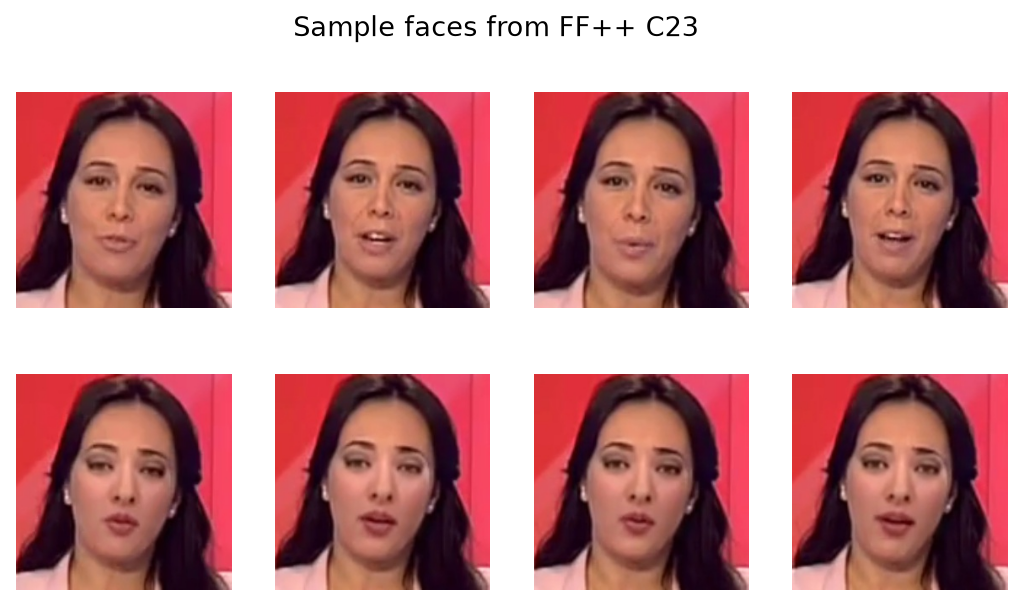
\includegraphics[width=0.92\linewidth]{fig_samples.png}
\caption{FF++ C23 中的人脸样本（上排真、下排假）}
\label{fig:samples}
\end{figure}

\subsection{身份隔离划分}

按源视频 id 分组划分，初始为 280/60/60 个身份，扩展后为 580/60/60。验证集用于选模型与选阈值，测试集只在最终评估时使用。每次划分后检查训练集与测试集的身份交集，必须为 0。

\subsection{退化生成}

为模拟真实传播链，本文实现 6 类退化，见表~\ref{tab:degrade}。训练时以 50\% 概率随机施加 1--2 种退化，评测时按固定参数施加。

\begin{table}[H]
\centering
\caption{评测使用的退化类型}
\label{tab:degrade}
\small
\begin{tabular}{lll}
\toprule
退化 & 参数 & 模拟场景 \\
\midrule
JPEG 重压缩 & 质量 70/50/30 & 社交平台二次压缩 \\
高斯噪声 & $\sigma=5$ & 低质量采集、传输噪声 \\
高斯模糊 & $5\times5$ & 失焦、运动模糊 \\
下采样 & 0.5 倍后再放大 & 低分辨率 \\
随机裁剪 & 裁剪 10\% 后放大 & 构图裁剪、缩放 \\
干净 & 原图 & 对照 \\
\bottomrule
\end{tabular}
\end{table}

\subsection{评测指标与两套口径}

单一阈值下的指标容易掩盖问题，本文同时报告两套口径：

\begin{itemize}
  \item \textbf{部署口径}：用验证集选出的冻结阈值，报告 F1、召回、FPR。阈值在测试集与跨库数据上\textbf{绝不重调}。
  \item \textbf{排序口径}：在测试集 ROC 上取 FPR=1\% 与 FPR=10\% 对应的 TPR（TPR@FPR1\%、TPR@FPR10\%），衡量与阈值无关的排序能力。
\end{itemize}

此外报告 AUC、EER，并对视频做 20 帧平均后的\textbf{视频级}指标。

\subsection{数据规模}

\begin{table}[H]
\centering
\caption{数据规模对比（测试集保持不变，保证可比）}
\label{tab:scale}
\small
\begin{tabular}{lcc}
\toprule
项 & 初始 & 扩展后 \\
\midrule
训练身份 & 280 & 580 \\
验证/测试身份 & 60 / 60 & 60 / 60（不变） \\
训练帧 & 16,800 & 34,719 \\
训练真假比 & 1:2 & 1:2 \\
测试帧 & 3,600（180 条视频） & 3,600（不变） \\
\bottomrule
\end{tabular}
\end{table}

\subsection{处理流程}

图~\ref{fig:pipeline} 给出了从原始视频到评测的完整流程。

\begin{figure}[H]
\centering
\begin{tikzpicture}[
  node distance=6mm,
  box/.style={draw, rounded corners=2pt, align=center, minimum height=9mm, font=\small, fill=gray!6},
  arr/.style={-{Stealth[length=2mm]}, thick}
]
\node[box] (v) {原始视频\\（FF++ C23）};
\node[box, right=of v] (f) {抽帧\\2 fps};
\node[box, right=of f] (c) {YuNet 裁脸\\256$\times$256};
\node[box, right=of c] (s) {按身份\\划分};
\node[box, below=of s] (tr) {训练集\\580 身份};
\node[box, left=of tr] (va) {验证集\\60 身份};
\node[box, left=of va] (te) {测试集\\60 身份};
\node[box, below=of tr] (deg) {随机退化\\50\% 概率};
\node[box, left=of deg] (m) {ResNet18\\训练};
\node[box, left=of m] (e) {多口径评测\\同库/跨库/退化};
\draw[arr] (v) -- (f);
\draw[arr] (f) -- (c);
\draw[arr] (c) -- (s);
\draw[arr] (s) -- (tr);
\draw[arr] (s) -- (va);
\draw[arr] (s) -- (te);
\draw[arr] (tr) -- (deg);
\draw[arr] (deg) -- (m);
\draw[arr] (m) -- (e);
\end{tikzpicture}
\caption{数据处理与评测流程}
\label{fig:pipeline}
\end{figure}

\section{方法}

\subsection{总体框架}

输入 224$\times$224 人脸图，RGB 分支与频域分支分别提取特征，拼接后经全连接层输出二分类 logits，softmax 得到伪造概率。频域分支前接一个质量感知门控，按图像高频能量调整其权重。整体结构如图~\ref{fig:arch} 所示。

\begin{figure}[H]
\centering
\begin{tikzpicture}[
  node distance=7mm and 9mm,
  box/.style={draw, rounded corners=2pt, align=center, minimum height=8mm, font=\small, fill=gray!6},
  op/.style={draw, circle, inner sep=1pt, font=\small, fill=white},
  arr/.style={-{Stealth[length=2mm]}, thick}
]
\node[box] (in) {输入\\224$\times$224};
\node[box, right=of in] (rgb) {ResNet18\\（预训练）};
\node[box, right=of rgb] (f512) {512 维};
\node[box, below=14mm of in] (fft) {FFT + SRM\\4 通道};
\node[box, right=of fft] (cnn) {4 层 CNN\\+ GAP};
\node[box, right=of cnn] (f256) {256 维};
\node[box, below=10mm of f256] (gate) {质量门控\\$g=\sigma(\mathrm{MLP}(q))$};
\node[op, right=of f512] (cat) {$\oplus$};
\node[box, right=of cat] (fc) {FC 256\\$\to$ 2};
\node[box, right=of fc] (out) {softmax\\$p(\text{fake})$};
\draw[arr] (in) -- (rgb);
\draw[arr] (rgb) -- (f512);
\draw[arr] (in.south) -- (fft.north);
\draw[arr] (fft) -- (cnn);
\draw[arr] (cnn) -- (f256);
\draw[arr, dashed] (gate.north) -- node[right,font=\scriptsize]{$\times$} (f256.south);
\draw[arr] (f512) -- (cat);
\draw[arr] (f256) -- (cat);
\draw[arr] (cat) -- (fc);
\draw[arr] (fc) -- (out);
\end{tikzpicture}
\caption{双流检测模型结构（虚线表示门控对频域特征的缩放）}
\label{fig:arch}
\end{figure}

\subsection{RGB 分支}

采用 ImageNet 预训练的 ResNet18，去掉最后的全连接层，输出 512 维特征。选择 ResNet18 的原因是：数据规模中等、8 GB 显存可训练、推理快（单图毫秒级），便于系统落地。迁移学习缓解了小数据下的过拟合。

\subsection{频域分支}

对灰度图做二维 FFT，取幅度谱并做 $\log(1+|\cdot|)$ 压缩动态范围，再逐图 z-score 标准化；同时用 SRM 高通滤波器提取噪声残差（3 个 $5\times5$ 固定核，不参与训练）。两者拼接为 4 通道输入，经 4 层卷积 + 全局平均池化得到 256 维特征。

设计动机：伪造过程中的上采样、插值、生成器上采样层会在频域留下痕迹；SRM 残差则抑制图像内容、突出噪声层面的伪造线索。

\subsection{质量感知门控}

设图像高频能量为
\begin{equation}
  h_f = \frac{1}{HW}\sum_{i,j}\left|\,g_{ij} - \mathrm{avgpool}_{3\times3}(g)_{ij}\,\right|,
\end{equation}
其中 $g$ 为灰度图。门控值定义为
\begin{equation}
  q = \log(1 + 10 h_f), \qquad
  \gamma = \sigma\!\left(W_2\,\mathrm{ReLU}(W_1 q + b_1) + b_2\right),
\end{equation}
频域特征被缩放为 $\tilde{f} = \gamma \cdot f_{\text{freq}}$。

直觉是：图像清晰（高频高）时频域特征可信，门控接近 1；图像被压糊时门控接近 0，自动降低频域分支权重。第 5 章将说明该设计在本数据上失效的原因。

\subsection{训练策略}

\begin{itemize}
  \item 损失：交叉熵 + 类别加权（真 1.5、假 0.75，缓解 1:2 不平衡）；
  \item 优化器：AdamW，学习率 $10^{-4}$，weight decay $10^{-4}$，cosine 退火，15 epoch；
  \item 混合精度训练，batch size 32；
  \item 数据增强：随机水平翻转 + 50\% 概率随机退化；
  \item 模型选择：按\textbf{验证集 AUC}（而非 F1），避免阈值依赖带来的选择噪声；
  \item 早停：验证 AUC 连续 4 轮不涨则停止。
\end{itemize}

\subsection{阈值选择}

训练结束后在验证集上计算两个阈值：满足 FPR$\le$1\% 的阈值（部署默认），以及使 F1 最大的阈值（报告对照），一并写入 checkpoint。跨库评测沿用源域阈值，不做任何调整。

\section{实验与结果}

\subsection{实验设置}

硬件为 RTX 4060 Laptop（8 GB），PyTorch 2.15。除非特别说明，模型均为 RGB 基线、580 个训练身份、3,600 帧测试集。训练曲线见图~\ref{fig:train}。

\begin{figure}[H]
\centering
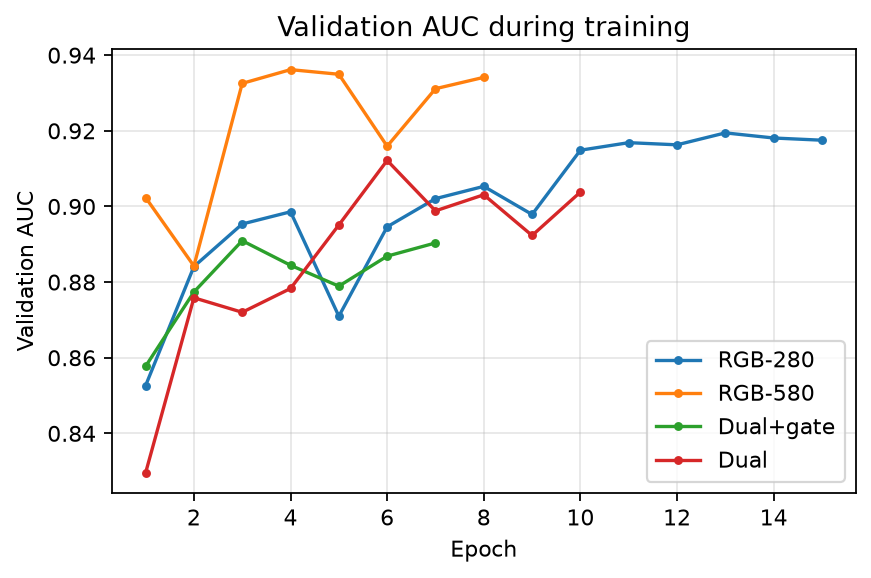
\includegraphics[width=0.72\linewidth]{fig_training_curve.png}
\caption{各模型验证集 AUC 随训练轮次的变化}
\label{fig:train}
\end{figure}

\subsection{同库结果}

\begin{table}[H]
\centering
\caption{同库结果（测试集 3,600 帧 / 180 条视频）}
\label{tab:indomain}
\scriptsize
\setlength{\tabcolsep}{3.5pt}
\begin{tabular}{lcccccc}
\toprule
\multirow{2}{*}{模型} & \multicolumn{2}{c}{帧级} & \multicolumn{2}{c}{视频级} & \multirow{2}{*}{F1@0.5} & \multirow{2}{*}{FPR@0.5} \\
\cmidrule(lr){2-3}\cmidrule(lr){4-5}
 & AUC & TPR@1\% & AUC & TPR@1\% & & \\
\midrule
E1 RGB-8ep & 0.8763 & 0.231 & -- & -- & 0.850 & 24.0\% \\
E2 RGB-280 & 0.9115 & 0.365 & 0.9308 & 0.425 & 0.870 & 16.6\% \\
\textbf{E9 RGB-580} & \textbf{0.9328} & \textbf{0.596} & \textbf{0.9499} & \textbf{0.700} & \textbf{0.886} & 10.5\% \\
\bottomrule
\end{tabular}
\end{table}

E1 暴露了两个问题：训练时 100\% 加退化、测试是干净图，分布不匹配；且按 F1@FPR1\% 选模型噪声大。E2 把退化概率降到 50\%、改按 AUC 选模型、加类别权重，AUC 提升 0.057。E9 把训练身份从 280 扩到 580，AUC 再提升 0.021，低误报召回提升 23 个百分点，说明数据量是此前的瓶颈之一。

\subsection{双流与门控消融}

\begin{table}[H]
\centering
\caption{双流与门控消融}
\label{tab:ablation}
\small
\begin{tabular}{lccc}
\toprule
模型 & 帧级 AUC & 视频级 AUC & 跨库 AUC \\
\midrule
RGB（E2） & 0.9115 & 0.9308 & 0.6687 \\
双流 + 门控（E3） & 0.9088 & \textbf{0.9411} & 0.6666 \\
双流无门控（E3b） & 0.9067 & 0.9297 & 0.6823 \\
\bottomrule
\end{tabular}
\end{table}

三者差异在 $\pm 0.011$ 内且互有胜负，属于划分与随机种子噪声。\textbf{频域分支未带来稳定收益。}

\textbf{门控失效分析}：在 1,408 张测试图上统计，门控输出均值 0.4272、标准差 \textbf{0.0008}，真图 0.4274、假图 0.4271，几乎是一个常数（图~\ref{fig:gate}）。原因有两层：其一，门控输入 $\log(1+10h_f)$ 中 $h_f$ 仅约 0.005，输入变化范围不足 0.01；其二，真假图的高频能量分布几乎完全重叠（真 $0.0053\pm0.0010$，假 $0.0049$--$0.0058$），该“质量代理”本身没有区分度。因此门控不是“没训好”，而是设计前提不成立。

\begin{figure}[H]
\centering
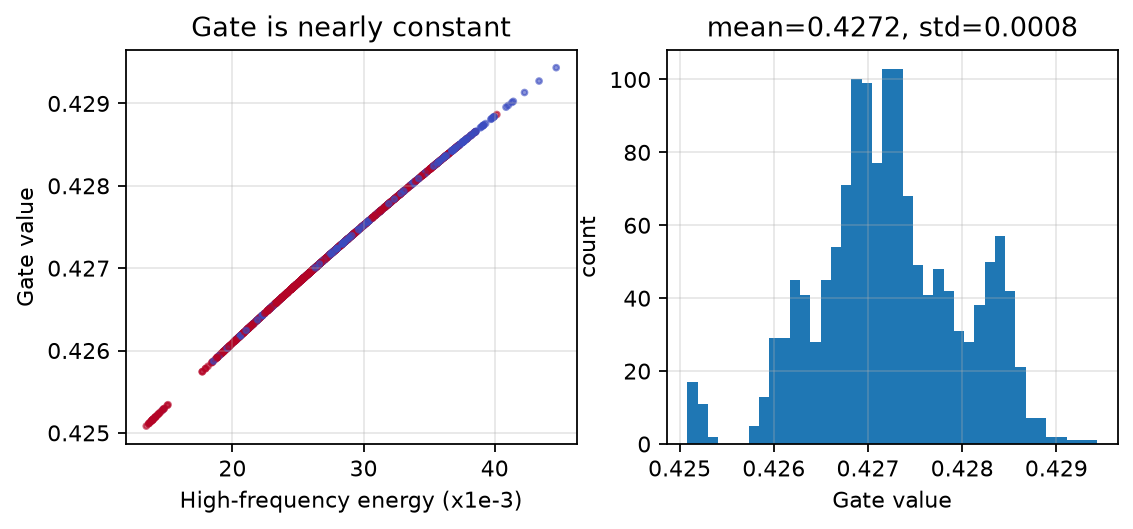
\includegraphics[width=0.9\linewidth]{fig_gate.png}
\caption{门控值随高频能量的变化（左）与分布（右）：几乎恒为 0.427}
\label{fig:gate}
\end{figure}

\textbf{频谱分析}：对 200 张真图与 200 张假图求平均 log 幅度谱并相减，差异集中在水平与垂直两条轴上，呈明显十字形（图~\ref{fig:specdiff}），其余区域接近噪声。轴对齐的强差异更符合 JPEG $8\times8$ 块效应与重采样的形态，而非生成器指纹。这解释了频域分支为何同库不涨、跨库不迁移。

\begin{figure}[H]
\centering
\begin{subfigure}{0.31\linewidth}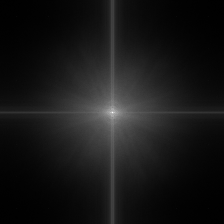
\includegraphics[width=\linewidth]{spectrum_real.png}\caption{真图平均谱}\end{subfigure}
\hfill
\begin{subfigure}{0.31\linewidth}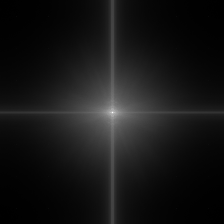
\includegraphics[width=\linewidth]{spectrum_fake.png}\caption{假图平均谱}\end{subfigure}
\hfill
\begin{subfigure}{0.31\linewidth}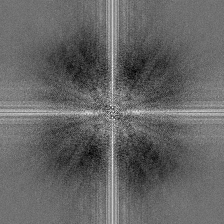
\includegraphics[width=\linewidth]{spectrum_diff.png}\caption{差异（假$-$真）}\end{subfigure}
\caption{真假平均频谱与差异：差异呈轴对齐十字形，更像压缩块效应}
\label{fig:specdiff}
\end{figure}

\subsection{鲁棒性矩阵}

\begin{table}[H]
\centering
\caption{主模型（RGB-580）在不同退化下的表现（冻结阈值）}
\label{tab:robust}
\small
\begin{tabular}{lccccc}
\toprule
退化 & AUC & F1 & 召回 & FPR & TPR@1\% \\
\midrule
干净 & 0.9328 & 0.652 & 0.484 & 0.33\% & 0.596 \\
JPEG 70 & 0.9123 & 0.664 & 0.500 & 1.25\% & 0.493 \\
JPEG 50 & 0.8896 & 0.633 & 0.467 & 1.67\% & 0.394 \\
JPEG 30 & 0.8617 & 0.540 & 0.372 & 1.25\% & 0.363 \\
噪声 $\sigma=5$ & 0.8984 & 0.529 & 0.360 & 0.58\% & 0.484 \\
模糊 $5\times5$ & 0.8933 & 0.424 & 0.270 & 0.33\% & 0.353 \\
下采样 0.5 & 0.8988 & 0.471 & 0.309 & 0.67\% & 0.354 \\
裁剪 10\% & 0.9180 & 0.575 & 0.405 & 0.58\% & 0.471 \\
\bottomrule
\end{tabular}
\end{table}

\begin{figure}[H]
\centering
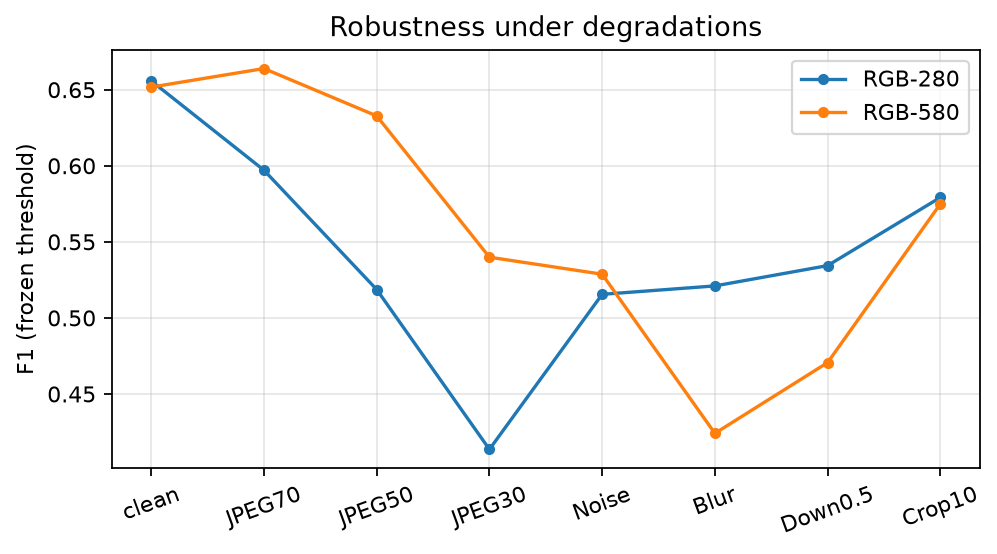
\includegraphics[width=0.78\linewidth]{fig_robustness.png}
\caption{两种训练规模下的鲁棒性曲线}
\label{fig:robust}
\end{figure}

与 280 身份版本相比，JPEG 鲁棒性明显改善（JPEG30 掉点从 24.2 pt 降到 11.2 pt），但模糊与下采样变差，说明模型仍依赖高频细节。TPR@1\% 在所有退化下都下降，表明排序能力本身受损，不只是阈值漂移。

\subsection{跨库结果}

\begin{table}[H]
\centering
\caption{跨库 Celeb-DF 结果（阈值冻结）}
\label{tab:cross}
\small
\begin{tabular}{lccc}
\toprule
模型 & 跨库 AUC & 跨库 TPR@1\% & 跨库 TPR@10\% \\
\midrule
E2（280 身份） & 0.6687 & 0.041 & -- \\
E9（580 身份） & \textbf{0.7163} & 0.068 & 0.281 \\
\bottomrule
\end{tabular}
\end{table}

扩数据让跨库 AUC 提升 0.048，说明更多身份带来了一点更通用的线索；但 0.716 仍不足以称为“跨库可用”，域偏移问题没有解决。冻结阈值下跨库 F1 很低，再次说明源域阈值不能直接迁移。图~\ref{fig:roc} 给出了主模型在同库与跨库上的 ROC 曲线。

\begin{figure}[H]
\centering
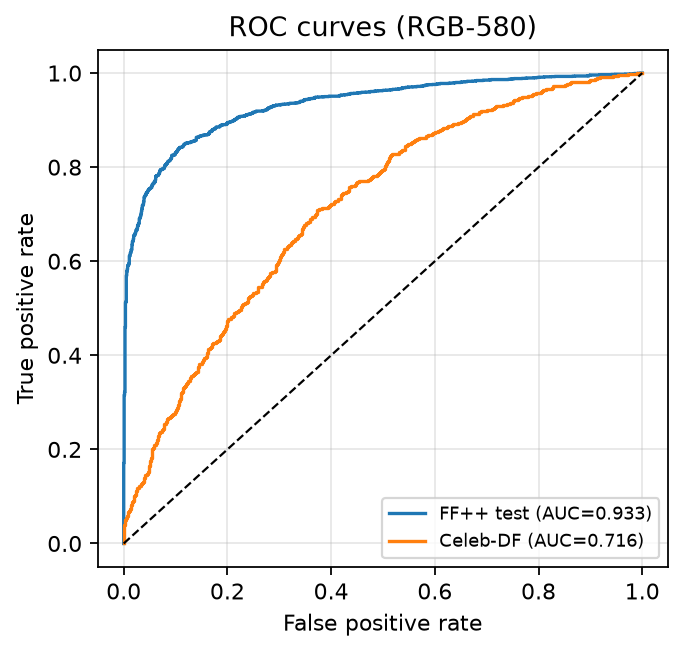
\includegraphics[width=0.55\linewidth]{fig_roc.png}
\caption{同库与跨库 ROC 曲线}
\label{fig:roc}
\end{figure}

\begin{figure}[H]
\centering
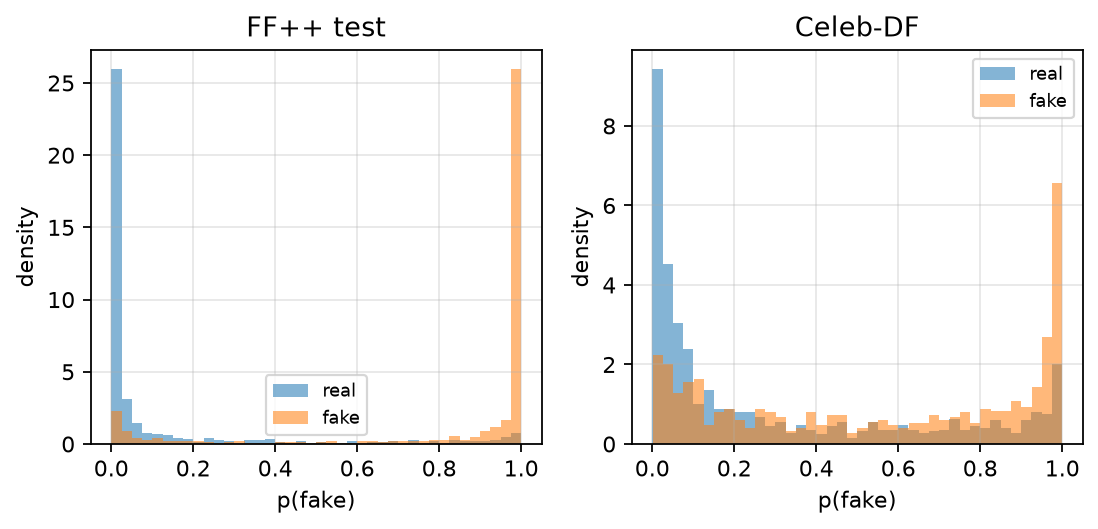
\includegraphics[width=0.85\linewidth]{fig_score_dist.png}
\caption{真、假样本的分数分布（左：FF++；右：Celeb-DF）}
\label{fig:dist}
\end{figure}

\subsection{未见伪造方法}

训练时完全移除 FaceShifter，测试集只含真人 + FaceShifter：

\begin{table}[H]
\centering
\caption{未见方法（FaceShifter）泛化}
\label{tab:unseen}
\small
\begin{tabular}{lccc}
\toprule
训练身份 & AUC & TPR@1\% & TPR@10\% \\
\midrule
280 & 0.5463 & 0.000 & 0.053 \\
580 & 0.5975 & 0.000 & 0.087 \\
\bottomrule
\end{tabular}
\end{table}

数据量翻倍只把 AUC 从 0.546 提到 0.598，1\% 误报下仍抓不到任何一张。对比同库 TPR@1\% 从 0.365 提到 0.596、跨库 AUC 从 0.669 提到 0.716，可见\textbf{扩数据改善“见过的类型”和“域内差异”，但解决不了“没见过的生成方法”}。后者是捷径学习问题。

\subsection{可解释性}

\textbf{Grad-CAM}：对 RGB 分支最后一层卷积做梯度加权，热图集中在眼、鼻、口区域（图~\ref{fig:cam}），定性合理。

\begin{figure}[H]
\centering
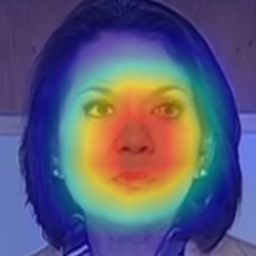
\includegraphics[width=0.34\linewidth]{heatmap_example.png}
\caption{Grad-CAM 热图示例}
\label{fig:cam}
\end{figure}

\textbf{定量 faithfulness}：取 100 张判为假的图，按热图从高到低遮挡（deletion）或只露出（insertion），被遮像素用强模糊图填充，与 3 组随机顺序对比，11 档遮挡比例，计算归一化概率曲线面积：

\begin{table}[H]
\centering
\caption{deletion / insertion 定量对比}
\label{tab:faith}
\small
\begin{tabular}{lccc}
\toprule
指标 & CAM & 随机 & 说明 \\
\midrule
deletion AUC（越低越好） & \textbf{1.037} & 1.259 & CAM 区域更关键 \\
insertion AUC（越高越好） & \textbf{1.324} & 1.254 & CAM 区域能更快恢复伪造分数 \\
\bottomrule
\end{tabular}
\end{table}

两项均优于随机，说明热图确实携带判定信息；但绝对 AUC 大于 1，是因为模糊填充本身会推高伪造分数，因此只能做相对比较，不能当作绝对解释质量。

\subsection{讨论：证据链}

四组实验指向同一结论：

\begin{enumerate}
  \item 门控退化为常数 $\rightarrow$ 质量代理无区分度；
  \item 频谱差异呈压缩块效应形态 $\rightarrow$ 频域分支学的是压缩方式；
  \item 强压缩下 F1 掉 11--23 pt $\rightarrow$ 依赖高频线索；
  \item 未见方法 AUC 0.598 $\rightarrow$ 学到的是训练方法的指纹。
\end{enumerate}

因此，同库 0.93 的 AUC 有相当一部分来自捷径；这也解释了为什么跨库、强压缩、未见方法三处同时失效。该结论与 DF40 的观察一致：在过时的 FF++ 上训练、只做闭集评测，会高估真实能力。

\subsection{与现有工作的性能差距}

本文主模型的实测指标与公开结果对比如表~\ref{tab:gap} 所示。

\begin{table}[H]
\centering
\caption{与代表性工作的性能对比（FF++ c23 / Celeb-DF）}
\label{tab:gap}
\small
\begin{tabular}{lccc}
\toprule
方法 & 训练规模 & FF++ c23 ACC & Celeb-DF AUC \\
\midrule
Xception\cite{rossler2019ffpp} & 全量 FF++ & 约 95.7\% & 约 0.65--0.70 \\
F3-Net\cite{qian2020f3net} & 全量 FF++ & 约 97.5\% & 约 0.65--0.75 \\
SPSL\cite{liu2021spsl} & 全量 FF++ & 约 99\% & 约 0.76 \\
ICT\cite{dong2022ict} & 全量 FF++ & -- & 约 0.86 \\
\midrule
本文（RGB-580） & 580 身份 / 3.5 万帧 & 85.6\% & 0.716 \\
\bottomrule
\end{tabular}
\end{table}

需要强调，这张表只能看量级，不能逐项比较：公开方法通常使用 720 个以上身份、数十万到百万级训练帧、
Xception/EfficientNet 级 backbone，并在视频级做评测；本文使用 580 个身份、约 3.5 万帧、ResNet18，
测试集只有 60 个身份、3,600 帧，且训练与测试身份完全隔离，难度更高。

差距的主要来源有四点：

\begin{enumerate}
  \item \textbf{数据规模}：本文训练帧数约为常用设置的十分之一到几十分之一；
  \item \textbf{模型容量}：ResNet18 小于 Xception/EfficientNet，且未做视频时序建模；
  \item \textbf{评测协议}：身份隔离 + 仅 60 个测试身份，比随机划分更难，尾部指标方差也更大；
  \item \textbf{伪造类型}：测试包含 NeuralTextures、FaceShifter 等弱伪影方法，拉低整体指标。
\end{enumerate}

在阈值 0.5 时，本文 ACC 85.6\%、F1 0.886、FPR 10.5\%；若压到 FPR$\le$1\% 的严格阈值，
ACC 降到 65.5\%、召回 48.4\%。这说明模型的主要短板在低误报区间，而不是整体排序能力。

\section{系统设计与实现}

\subsection{架构}

系统采用“推理核心 + Web 服务 + 报告生成 + 审计”四层结构：

\begin{itemize}
  \item \texttt{app/detector.py}：模型加载、YuNet 人脸裁剪、打分、Grad-CAM、频谱；
  \item \texttt{app/main.py}：FastAPI 路由、文件落盘、结果 JSON；
  \item \texttt{app/report.py} + \texttt{app/templates/report.html}：Jinja2 渲染 HTML，WeasyPrint 转 PDF；
  \item \texttt{app/audit.py}：JSONL 哈希链审计日志。
\end{itemize}

\subsection{接口}

\begin{table}[H]
\centering
\caption{系统接口}
\label{tab:api}
\small
\begin{tabular}{lll}
\toprule
方法 & 路径 & 功能 \\
\midrule
GET & \texttt{/} & 单页上传界面 \\
POST & \texttt{/v1/detect/image} & 返回分数、判定、热图/频谱 URL、审计哈希 \\
GET & \texttt{/v1/report/\{id\}.pdf} & 单页 A4 PDF 报告 \\
GET & \texttt{/v1/audit/verify} & 校验审计日志完整性 \\
GET & \texttt{/healthz} & 健康检查 \\
\bottomrule
\end{tabular}
\end{table}

\subsection{审计设计}

每条日志记录包含 \texttt{prev\_hash} 与 \texttt{hash}，其中
\[
  \mathrm{hash} = \mathrm{SHA256}\big(\mathrm{prev\_hash} \,\|\, \mathrm{canonical(record)}\big).
\]
任意一条被篡改，后续哈希全部对不上，\texttt{/v1/audit/verify} 即可发现。报告内嵌输入文件的 SHA-256，便于追溯。

\subsection{界面与报告}

图~\ref{fig:ui} 与图~\ref{fig:pdf} 为系统界面与报告截图。

\begin{figure}[H]
\centering
\screenshot{fig_ui.png}{Web 界面：拖拽上传、伪造概率、Grad-CAM 热图、频谱图、PDF 下载}
\caption{系统 Web 界面}
\label{fig:ui}
\end{figure}

\begin{figure}[H]
\centering
\screenshot{fig_pdf.png}{PDF 报告：判定结果、元信息、三张图、审计哈希}
\caption{PDF 审计报告}
\label{fig:pdf}
\end{figure}

\subsection{性能}

\begin{table}[H]
\centering
\caption{系统性能实测}
\label{tab:perf}
\small
\begin{tabular}{lc}
\toprule
项 & 结果 \\
\midrule
单图推理（热启动，含人脸检测） & 10.9 ms \\
单图推理（冷启动） & 276.5 ms \\
批量 10 张（模型加载后） & 17.3 ms/张 \\
PDF 生成 & 单页约 517 KB \\
审计链校验 & 通过 \\
\bottomrule
\end{tabular}
\end{table}

\subsection{演示流程}

上传图片 $\rightarrow$ 显示伪造概率、热图、频谱 $\rightarrow$ 下载 PDF。系统默认使用主模型 \texttt{runs/rgb\_700}，阈值固定为验证集 F1 最优值；FPR$\le$1\% 的严格阈值仅用于结果对照，不在界面暴露。

\section{总结与展望}

\subsection{工作总结}

本文完成了一套图像级深度伪造检测的完整流程：按身份隔离的数据管线、RGB 基线、双流与门控、多维度评测、可解释性验证和可演示系统。主要结论是：

\begin{enumerate}
  \item 数据量对同库性能影响显著（280$\to$580 身份，AUC $+0.021$，TPR@1\% $+23$ pt）；
  \item 频域分支与质量门控在本数据上没有稳定收益，门控退化为常数；
  \item 真假频谱差异主要来自压缩块效应，而非生成器指纹；
  \item 未见伪造方法上模型接近随机，存在明显的捷径学习；
  \item 系统在单图 11 ms 下可完成检测、解释与报告生成。
\end{enumerate}

\subsection{局限性}

\begin{itemize}
  \item 数据仅覆盖 FF++ C23 的 5 种方法，未包含扩散生成与商用工具；
  \item 图像级检测，未利用视频时序与音频；
  \item 门控设计过于简单，未验证多维质量描述子；
  \item 跨库与开集泛化仍是短板；
  \item 未做多随机种子重复，部分差异可能落在噪声范围内。
\end{itemize}

\subsection{未来工作}

\begin{itemize}
  \item 引入 SBI 等自混合增广，提升对未见方法的泛化；
  \item 测试时 BN 适应 / 域适应，缓解跨库偏移；
  \item 用多维质量描述子（高频能量 + 噪声估计 + 模糊度）重做门控；
  \item 扩展到视频时序与多模态；
  \item 结合重构误差（DIRE/AEROBLADE）做通用 AIGC 检测。
\end{itemize}


\subsection*{人工智能工具使用声明}

本文在完成过程中使用了人工智能辅助工具（DeepSeek Harness 及其调用的 DeepSeek V4.1 Flash 模型），
主要用于以下环节：

\begin{enumerate}
  \item 代码实现与调试：数据处理、训练与评测脚本、Web 演示系统的编写与问题定位；
  \item 实验整理：实验结果的汇总、图表生成脚本的编写；
  \item 文献与写作：相关工作的检索线索、报告初稿的文字组织与 \LaTeX{} 排版。
\end{enumerate}

所有研究问题的设定、数据选择、实验方案、结果解读与结论均由作者确认并对内容负责；
AI 生成的代码与文字均经过人工检查、修改与验证。文中如有错误，责任由作者承担。


\begin{thebibliography}{99}

\bibitem{goodfellow2014gan} Goodfellow I, Pouget-Abadie J, Mirza M, et al. Generative Adversarial Nets[C]. Advances in Neural Information Processing Systems (NeurIPS), 2014.

\bibitem{rossler2019ffpp} Rossler A, Cozzolino D, Verdoliva L, et al. FaceForensics++: Learning to Detect Manipulated Facial Images[C]. IEEE/CVF International Conference on Computer Vision (ICCV), 2019.

\bibitem{li2020celebd} Li Y, Yang X, Sun P, et al. Celeb-DF: A Large-Scale Challenging Dataset for DeepFake Forensics[C]. IEEE/CVF Conference on Computer Vision and Pattern Recognition (CVPR), 2020.

\bibitem{dolhansky2020dfdc} Dolhansky B, Bitton J, Pflaum B, et al. The DeepFake Detection Challenge (DFDC) Dataset[J]. arXiv:2006.07397, 2020.

\bibitem{afchar2018mesonet} Afchar D, Nozick V, Yamagishi J, et al. MesoNet: a Compact Facial Video Forgery Detection Network[C]. IEEE International Workshop on Information Forensics and Security (WIFS), 2018.

\bibitem{qian2020f3net} Qian Y, Yin G, Sheng L, et al. Thinking in Frequency: Face Forgery Detection by Mining Frequency-Aware Clues[C]. European Conference on Computer Vision (ECCV), 2020.

\bibitem{liu2021spsl} Liu H, Li X, Zhou W, et al. Spatial-Phase Shallow Learning: Rethinking Face Forgery Detection in Frequency Domain[C]. IEEE/CVF Conference on Computer Vision and Pattern Recognition (CVPR), 2021.

\bibitem{luo2021srm} Luo Y, Zhang Y, Yan J, et al. Generalizing Face Forgery Detection with High-Frequency Features[C]. IEEE/CVF Conference on Computer Vision and Pattern Recognition (CVPR), 2021.

\bibitem{zhao2021multi} Zhao H, Zhou W, Chen D, et al. Multi-Attentional Deepfake Detection[C]. IEEE/CVF Conference on Computer Vision and Pattern Recognition (CVPR), 2021.

\bibitem{cao2022recce} Cao J, Ma C, Yao T, et al. End-to-End Reconstruction-Classification Learning for Face Forgery Detection[C]. IEEE/CVF Conference on Computer Vision and Pattern Recognition (CVPR), 2022.

\bibitem{shiohara2022sbi} Shiohara K, Yamasaki T. Detecting Deepfakes with Self-Blended Images[C]. IEEE/CVF Conference on Computer Vision and Pattern Recognition (CVPR), 2022.

\bibitem{dong2022ict} Dong X, Bao J, Chen D, et al. Protecting Celebrities from DeepFake with Identity Consistency Transformer[C]. IEEE/CVF Conference on Computer Vision and Pattern Recognition (CVPR), 2022.

\bibitem{ojha2023univfd} Ojha U, Li Y, Lee Y J. Towards Universal Fake Image Detectors that Generalize Across Generative Models[C]. IEEE/CVF Conference on Computer Vision and Pattern Recognition (CVPR), 2023.

\bibitem{wang2023dire} Wang Z, Bao J, Zhou W, et al. DIRE for Diffusion-Generated Image Detection[C]. IEEE/CVF International Conference on Computer Vision (ICCV), 2023.

\bibitem{ricker2024aeroblade} Ricker J, Damm S, Holz T, et al. AEROBLADE: Training-Free Detection of Latent Diffusion Images Using Autoencoder Reconstruction Error[C]. IEEE/CVF Conference on Computer Vision and Pattern Recognition (CVPR), 2024.

\bibitem{yan2023deepfakebench} Yan Z, Zhang Y, Yuan X, et al. DeepfakeBench: A Comprehensive Benchmark of Deepfake Detection[C]. NeurIPS Datasets and Benchmarks, 2023.

\bibitem{yan2024df40} Yan Z, Yao T, Chen S, et al. DF40: Toward Next-Generation Deepfake Detection[J]. arXiv:2406.13495, 2024.

\bibitem{zhu2023genimage} Zhu M, Chen H, Yan Q, et al. GenImage: A Million-Scale Benchmark for Detecting AI-Generated Image[C]. NeurIPS Datasets and Benchmarks, 2023.

\bibitem{he2021forgerynet} He Y, Gan B, Chen S, et al. ForgeryNet: A Versatile Benchmark for Comprehensive Forgery Analysis[C]. IEEE/CVF Conference on Computer Vision and Pattern Recognition (CVPR), 2021.

\bibitem{jiang2020deeper} Jiang L, Li R, Wu W, et al. DeeperForensics-1.0: A Large-Scale Dataset for Real-World Face Forgery Detection[C]. IEEE/CVF Conference on Computer Vision and Pattern Recognition (CVPR), 2020.

\bibitem{thies2016face2face} Thies J, Zollh\"ofer M, Stamminger M, et al. Face2Face: Real-Time Face Capture and Reenactment of RGB Videos[C]. IEEE/CVF Conference on Computer Vision and Pattern Recognition (CVPR), 2016.

\bibitem{thies2019neural} Thies J, Zollh\"ofer M, Nie\ss{}ner M. Deferred Neural Rendering: Image Synthesis Using Neural Textures[J]. ACM Transactions on Graphics, 2019.

\bibitem{li2020faceshifter} Li L, Bao J, Yang H, et al. FaceShifter: Towards High Fidelity and Occlusion Aware Face Swapping[C]. IEEE/CVF Conference on Computer Vision and Pattern Recognition (CVPR), 2020.

\bibitem{ho2020ddpm} Ho J, Jain A, Abbeel P. Denoising Diffusion Probabilistic Models[C]. Advances in Neural Information Processing Systems (NeurIPS), 2020.

\bibitem{rombach2022ldm} Rombach R, Blattmann A, Lorenz D, et al. High-Resolution Image Synthesis with Latent Diffusion Models[C]. IEEE/CVF Conference on Computer Vision and Pattern Recognition (CVPR), 2022.

\bibitem{selvaraju2017gradcam} Selvaraju R R, Cogswell M, Das A, et al. Grad-CAM: Visual Explanations from Deep Networks via Gradient-Based Localization[C]. IEEE International Conference on Computer Vision (ICCV), 2017.

\bibitem{lin2023survey} 蔺琛皓, 沈超, 管晓宏, 等. 虚假数字人脸内容生成与检测技术[J]. 计算机学报.

\bibitem{cac2022deepsynth} 国家互联网信息办公室, 工业和信息化部, 公安部. 互联网信息服务深度合成管理规定[S]. 2022.

\bibitem{cac2023genai} 国家互联网信息办公室, 等. 生成式人工智能服务管理暂行办法[S]. 2023.

\bibitem{cac2025label} 国家互联网信息办公室, 工业和信息化部, 公安部, 国家广播电视总局. 人工智能生成合成内容标识办法[S]. 2025.

\end{thebibliography}


\end{document}
